This section presents the assessment of the model proposed in Section~\ref{sec:proposal} under different scenarios to measure the obtained C2 System agility. This assessment is performed through an \textit{in silico} experiment~\citep{simulation01} simulating UAVs dispatched on a reconnaissance mission to acquire images from a terrain. Such a method provides a way to analyze different situations and it allows us to work with different scenarios that would otherwise be unfeasible to test given incurred cost and resource availability. The simulated environment considers that the circumstances can change during the mission execution, allowing to test the effectiveness of the C2 System under such conditions. The replication package comprising the artifacts related to this empirical evaluation is available in a public repository.\footnote{\reproductibility}

The following sections present the goal definition and the metrics applied in the evaluation  (Section~\ref{ssec:definition}), the planning of the study  (Section~\ref{ssec:planning}), its execution (Section~\ref{subsec:operations}) and lastly, \X{analysis} of the obtained results and discussion about the findings  (Section~\ref{subsec:analysis_discussion}). 


 
%%%%%%%%%%%%%%%%%%%%%%%%%%%%%%%%%%
% SUBSECTION 
%%%%%%%%%%%%%%%%%%%%%%%%%%%%%%%%%%
\subsection{Definition}
\label{ssec:definition}

The performed empirical study is defined according to the Goal-Question-Metric (GQM)~\citep{gqm001} method. Figure~\ref{fig:gqm} shows the goal as the assessment of C2 Agility in our proposed computational model. The assessment made is useful to the entities' commanders. Such entities may be composed of internal entities, recursively, up to the level of individual members who also have commanders. From the goal, two research questions are derived, which consider the members within the same C2 Approach  (\textit{Q1}) and C2 Approach changes  (\textit{Q2}). Such questions address the level of C2 Agility existing in the system. Table \ref{table:metrics} defines the metrics applied in the evaluation to answer the proposed questions and corresponding agility enablers. The metrics are (\textit{M1 - Reconfigurations; M2 - Maneuvering; M3 - Engagement Time; M4 - Effectiveness; M5 - Resilience; M6 - Reward}) related to the agility enablers described by~\citet{Gren2019AgilityIR}, \citet{c2-02} and \citet{Alberts2011}.  


\begin{figure}[ht]
    \centering
    \scalebox{.52}{

\tikzset{every picture/.style={line width=0.75pt}} %set default line width to 0.75pt        

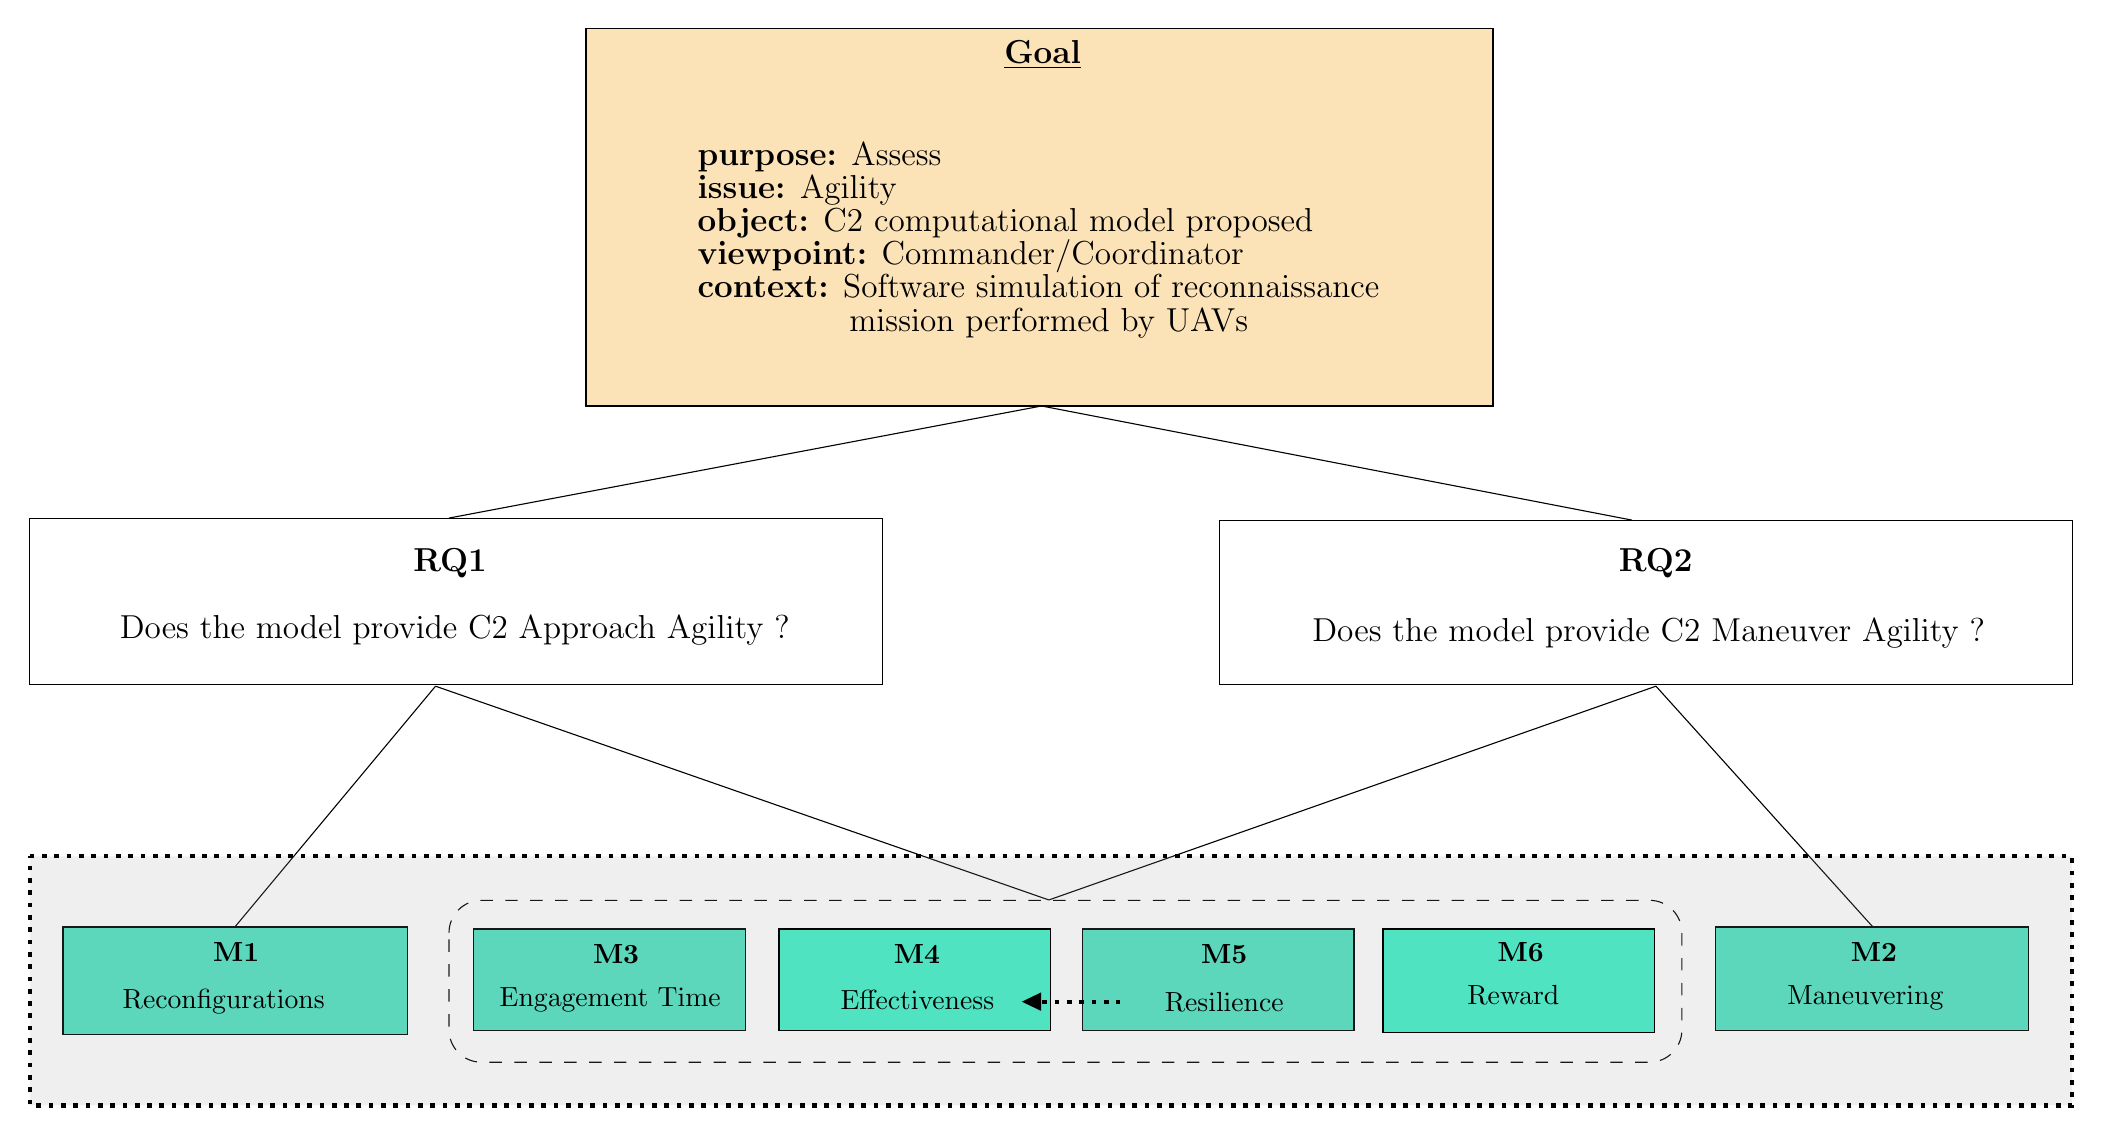
\begin{tikzpicture}[x=0.75pt,y=0.75pt,yscale=-1,xscale=1]
%uncomment if require: \path (0,532); %set diagram left start at 0, and has height of 532

%Flowchart: Process [id:dp9228173025001839] 
\draw  [fill={rgb, 255:red, 245; green, 166; blue, 35 }  ,fill opacity=0.33 ] (286.5,2) -- (723.5,2) -- (723.5,184) -- (286.5,184) -- cycle ;
%Shape: Rectangle [id:dp9468174970136011] 
\draw   (591.5,239) -- (1002.5,239) -- (1002.5,318) -- (591.5,318) -- cycle ;
%Shape: Rectangle [id:dp09665993774558346] 
\draw   (18.5,238) -- (429.5,238) -- (429.5,318) -- (18.5,318) -- cycle ;
%Straight Lines [id:da1961523796551078] 
\draw    (506,184) -- (220.5,238) ;
%Straight Lines [id:da6120336423295578] 
\draw    (506,184) -- (790.5,239) ;
%Shape: Rectangle [id:dp8704718643302001] 
\draw  [fill={rgb, 255:red, 80; green, 227; blue, 194 }  ,fill opacity=1 ] (232.5,436) -- (363.5,436) -- (363.5,485) -- (232.5,485) -- cycle ;
%Rounded Rect [id:dp2310824766673354] 
\draw  [dash pattern={on 4.5pt off 4.5pt}] (220.5,437.77) .. controls (220.5,429.15) and (227.48,422.17) .. (236.1,422.17) -- (798.9,422.17) .. controls (807.52,422.17) and (814.5,429.15) .. (814.5,437.77) -- (814.5,484.57) .. controls (814.5,493.18) and (807.52,500.17) .. (798.9,500.17) -- (236.1,500.17) .. controls (227.48,500.17) and (220.5,493.18) .. (220.5,484.57) -- cycle ;
%Straight Lines [id:da04635172987230718] 
\draw    (214,319) -- (116.5,436) ;
%Shape: Rectangle [id:dp16323070417268737] 
\draw  [fill={rgb, 255:red, 80; green, 227; blue, 194 }  ,fill opacity=1 ] (34.5,435) -- (200.5,435) -- (200.5,487) -- (34.5,487) -- cycle ;
%Straight Lines [id:da004791401702264886] 
\draw    (214,319) -- (509.5,422) ;
%Straight Lines [id:da9733307686397392] 
\draw    (802,319) -- (509.5,422) ;
%Straight Lines [id:da4492045519053316] 
\draw    (802,319) -- (906.5,435) ;
%Shape: Rectangle [id:dp7181001754521874] 
\draw  [fill={rgb, 255:red, 80; green, 227; blue, 194 }  ,fill opacity=1 ] (830.5,435) -- (981.5,435) -- (981.5,485) -- (830.5,485) -- cycle ;
%Shape: Rectangle [id:dp46797453967825375] 
\draw  [fill={rgb, 255:red, 80; green, 227; blue, 194 }  ,fill opacity=1 ] (525.5,436) -- (656.5,436) -- (656.5,485) -- (525.5,485) -- cycle ;
%Rounded Rect [id:dp9444454858651523] 
\draw  [fill={rgb, 255:red, 155; green, 155; blue, 155 }  ,fill opacity=0.16 ][dash pattern={on 1.69pt off 2.76pt}][line width=1.5]  (18.5,401) .. controls (18.5,401) and (18.5,401) .. (18.5,401) -- (1002.5,401) .. controls (1002.5,401) and (1002.5,401) .. (1002.5,401) -- (1002.5,521) .. controls (1002.5,521) and (1002.5,521) .. (1002.5,521) -- (18.5,521) .. controls (18.5,521) and (18.5,521) .. (18.5,521) -- cycle ;
%Shape: Rectangle [id:dp6205174536004793] 
\draw  [fill={rgb, 255:red, 80; green, 227; blue, 194 }  ,fill opacity=1 ] (379.5,436) -- (510.5,436) -- (510.5,485) -- (379.5,485) -- cycle ;
%Straight Lines [id:da0036921302300286785] 
\draw [line width=1.5]  [dash pattern={on 1.69pt off 2.76pt}]  (500.5,471) -- (544,471) ;
\draw [shift={(496.5,471)}, rotate = 0] [fill={rgb, 255:red, 0; green, 0; blue, 0 }  ][line width=0.08]  [draw opacity=0] (9.29,-4.46) -- (0,0) -- (9.29,4.46) -- cycle    ;
%Shape: Rectangle [id:dp36331169023965726] 
\draw  [fill={rgb, 255:red, 80; green, 227; blue, 194 }  ,fill opacity=1 ] (670.5,436) -- (801.5,436) -- (801.5,486) -- (670.5,486) -- cycle ;

% Text Node
\draw (506.5,15) node  [font=\normalsize] [align=left] {\textbf{\underline{{\large Goal}}}};
% Text Node
\draw (221,260) node   [align=left] {\textbf{{\large RQ1}}};
% Text Node
\draw (223.25,292) node   [align=left] {{\large Does the model provide C2 Approach Agility ?}};
% Text Node
\draw (798.5,293.5) node   [align=left] {{\large Does the model provide C2 Maneuver Agility ?}};
% Text Node
\draw (801.92,260) node   [align=left] {\textbf{{\large RQ2}}};
% Text Node
\draw (504.5,104) node   [align=left] {{\large \textbf{purpose:} Assess}\\{\large \textbf{issue:} Agility}\\{\large \textbf{object:} C2 computational model proposed}\\{\large \textbf{viewpoint:} Commander/Coordinator}\\{\large \textbf{context:} Software simulation of reconnaissance }\\{\large  \ \ \ \ \ \ \ \ \ \ \ \ \ \ mission performed by UAVs}};
% Text Node
\draw (301,448) node   [align=left] {\textbf{M3}};
% Text Node
\draw (118,447) node   [align=left] {\textbf{M1}};
% Text Node
\draw (907,447) node   [align=left] {\textbf{M2}};
% Text Node
\draw (298.17,470.17) node   [align=left] {Engagement Time};
% Text Node
\draw (594,448) node   [align=left] {\textbf{M5}};
% Text Node
\draw (446.17,470.17) node   [align=left] {Effectiveness};
% Text Node
\draw (446,448) node   [align=left] {\textbf{M4}};
% Text Node
\draw (594,471) node   [align=left] {Resilience};
% Text Node
\draw (62,464) node [anchor=north west][inner sep=0.75pt]   [align=left] {Reconfigurations};
% Text Node
\draw (864,462) node [anchor=north west][inner sep=0.75pt]   [align=left] {Maneuvering};
% Text Node
\draw (736.87,447) node   [align=left] {\textbf{M6}};
% Text Node
\draw (709.87,462) node [anchor=north west][inner sep=0.75pt]   [align=left] {Reward};


\end{tikzpicture}}
    \caption{GQM Diagram with the Goal, the Research Questions RQ1 and RQ2, and the metrics (M1, M2, M3, M4, M5 and M6)}
    \label{fig:gqm}
\end{figure}


\begin{table}[ht!]
	\small
	\fontsize{10}{10}\selectfont
	\centering
	\caption{Metrics used to evaluate the proposal}
	\label{table:metrics}
	
	\begin{tabularx}{\textwidth}{llXX}
	\hline
		\textbf{ID}
		& \textbf{Metric}
		& \textbf{Description} \\ [1ex]
	\hline	
	
	M1 & Reconfigurations & Number of internal reconfigurations performed by the members to accomplish the mission within a given timeout.
	\\[1ex] \\
	
	M2 & Maneuvering & Number of C2 Approach changes performed by the members to accomplish the mission within a given timeout.
	\\[1ex] \\
	
	M3 & Engagement Time & System time, in ticks, during which the entities were engaged in the execution of the tasks.
	\\[1ex] \\
	
	M4 & Effectiveness &  Percentage of successful tasks completed by the executors.
	\\[1ex] \\
	
	M5 & Resilience & System's capacity to obtain the same effectiveness of scenarios without context changes when dealing with new contexts.
	\\[1ex] \\
	
	M6 & Reward & Total quality of all sensors used to perform the tasks\\ 
	\\[1ex]
	\hline
	\end{tabularx}
\end{table} 


Context perturbations, e.g., sudden changes in the environment, or onboard component damage, require system adaptation to keep running. To identify the system's adaptation ability, the number of \color{black}member reconfigurations (M1) \color{black}and C2 Approach changes (M2) are counted. The Maneuvering (M2) metric assesses the adaptability level of the system due to its capability of \color{black} changing its organization. Response time \color{black} is measured by the Engagement Time (M3) metric, which measures how long the system takes to execute the mission's tasks. Such an aspect highlights the responsiveness of the system to changing circumstances. \X{ The Effectiveness (M4) metric evaluates the ratio of the mission’s tasks that the members have already accomplished with the total number of tasks.} 

The difference between the effectiveness (M4) metric obtained from scenarios with and without context changes shows the system capacity to recover the highest effectiveness level obtained from the scenario without context changes. Such recovery capacity defines the Resilience (M5) metric. Finally, Reward (M6) defines  the compatibility between the members and the \color{black}mission's tasks. \color{black}Equation~\ref{eq:reward} defines this metric in terms of the compatibility score $Q_{ij}$ sum.

\begin{equation}
    \label{eq:reward}
    M6=\sum Q_{ij} \ ,where\  t_j \in T_{success} \ and\ compatible(c_i,t_j)
\end{equation}

This score defines the compatibility level of a task $j$, which has a type, with a sensor $i$ used to perform it. Such a sensor corresponds to a feature in the configuration $c_i$ run by the member, and all tasks successfully performed are stored in $T_{success}$ for results analysis. Besides, all tasks with the same type have the same compatibility level to the sensors.


%%%%%%%%%%%%%%%%%%%%%%%%%%%%%%%%%%
% SUBSECTION 
%%%%%%%%%%%%%%%%%%%%%%%%%%%%%%%%%%
\subsection{Planning}
\label{ssec:planning}

The following sections describe the hypotheses on the proposed model (Section~\ref{sssec:hyp}), define the simulation scenarios  (Section~\ref{sssec:scenarios}), explain the experimental design and the analysis procedure (Section~\ref{sssec:design}), and the supporting instrumentation (Section~\ref{sssec:instrumentation}).


\subsubsection{Hypotheses Formulation}
\label{sssec:hyp}

Figure~\ref{fig:variables} shows the factors and the dependent variables related to the GQM (Figure~\ref{fig:gqm}). The scenario and the action method are identified as factors. A scenario comprises an initial context and a sequence of events that occur during the mission. Section~\ref{sssec:scenarios} details possible scenarios.

\begin{figure}[ht!]
    \centering
    \scalebox{.55}{

\tikzset{every picture/.style={line width=0.75pt}} %set default line width to 0.75pt        

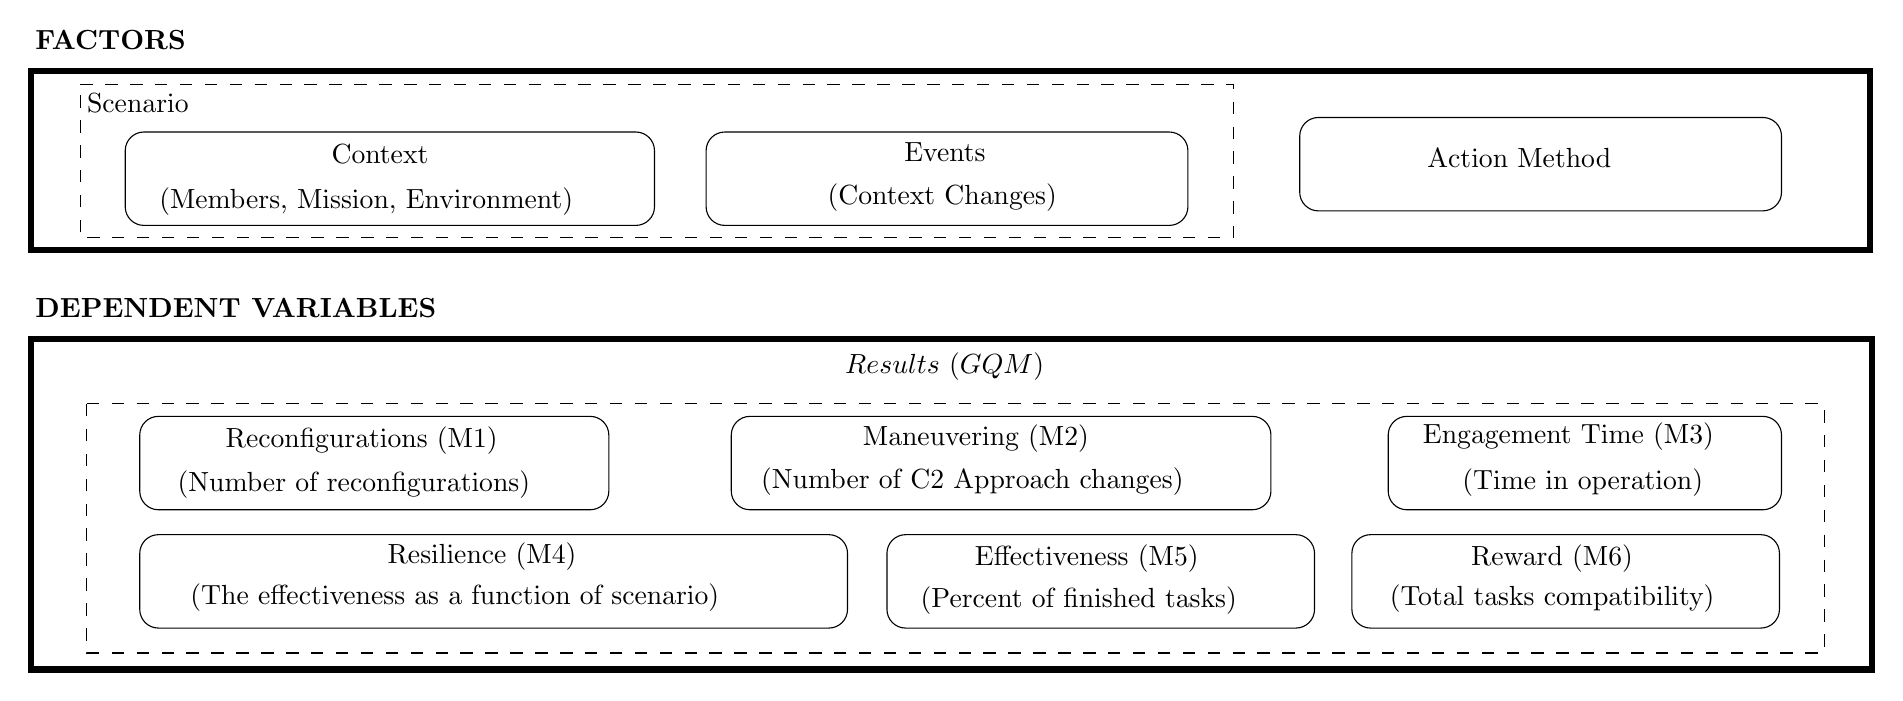
\begin{tikzpicture}[x=0.75pt,y=0.75pt,yscale=-1,xscale=1]
%uncomment if require: \path (0,322); %set diagram left start at 0, and has height of 322

%Rounded Rect [id:dp26709545620813635] 
\draw   (57.5,200) .. controls (57.5,195.03) and (61.53,191) .. (66.5,191) -- (274.5,191) .. controls (279.47,191) and (283.5,195.03) .. (283.5,200) -- (283.5,227) .. controls (283.5,231.97) and (279.47,236) .. (274.5,236) -- (66.5,236) .. controls (61.53,236) and (57.5,231.97) .. (57.5,227) -- cycle ;
%Shape: Rectangle [id:dp7868821488097882] 
\draw  [dash pattern={on 4.5pt off 4.5pt}] (32,185) -- (869,185) -- (869,305) -- (32,305) -- cycle ;
%Shape: Rectangle [id:dp07661178173797467] 
\draw  [line width=2.25]  (5,153.88) -- (892,153.88) -- (892,313) -- (5,313) -- cycle ;
%Rounded Rect [id:dp7819847156561298] 
\draw   (50.5,63) .. controls (50.5,58.03) and (54.53,54) .. (59.5,54) -- (296.5,54) .. controls (301.47,54) and (305.5,58.03) .. (305.5,63) -- (305.5,90) .. controls (305.5,94.97) and (301.47,99) .. (296.5,99) -- (59.5,99) .. controls (54.53,99) and (50.5,94.97) .. (50.5,90) -- cycle ;
%Shape: Rectangle [id:dp10398748207162001] 
\draw  [dash pattern={on 4.5pt off 4.5pt}] (28.85,31) -- (584.5,31) -- (584.5,105) -- (28.85,105) -- cycle ;
%Shape: Rectangle [id:dp48323694433186415] 
\draw  [line width=2.25]  (5,24.77) -- (891,24.77) -- (891,111) -- (5,111) -- cycle ;
%Rounded Rect [id:dp14086907660692627] 
\draw   (330.37,63) .. controls (330.37,58.03) and (334.4,54) .. (339.37,54) -- (553.5,54) .. controls (558.47,54) and (562.5,58.03) .. (562.5,63) -- (562.5,90) .. controls (562.5,94.97) and (558.47,99) .. (553.5,99) -- (339.37,99) .. controls (334.4,99) and (330.37,94.97) .. (330.37,90) -- cycle ;
%Rounded Rect [id:dp8800855997802748] 
\draw   (616.37,56) .. controls (616.37,51.03) and (620.4,47) .. (625.37,47) -- (839.5,47) .. controls (844.47,47) and (848.5,51.03) .. (848.5,56) -- (848.5,83) .. controls (848.5,87.97) and (844.47,92) .. (839.5,92) -- (625.37,92) .. controls (620.4,92) and (616.37,87.97) .. (616.37,83) -- cycle ;
%Rounded Rect [id:dp41591552385229413] 
\draw   (659,200) .. controls (659,195.03) and (663.03,191) .. (668,191) -- (839.5,191) .. controls (844.47,191) and (848.5,195.03) .. (848.5,200) -- (848.5,227) .. controls (848.5,231.97) and (844.47,236) .. (839.5,236) -- (668,236) .. controls (663.03,236) and (659,231.97) .. (659,227) -- cycle ;
%Rounded Rect [id:dp6557542326475674] 
\draw   (342.5,200) .. controls (342.5,195.03) and (346.53,191) .. (351.5,191) -- (593.5,191) .. controls (598.47,191) and (602.5,195.03) .. (602.5,200) -- (602.5,227) .. controls (602.5,231.97) and (598.47,236) .. (593.5,236) -- (351.5,236) .. controls (346.53,236) and (342.5,231.97) .. (342.5,227) -- cycle ;
%Rounded Rect [id:dp018207773722970888] 
\draw   (641.5,257) .. controls (641.5,252.03) and (645.53,248) .. (650.5,248) -- (838.5,248) .. controls (843.47,248) and (847.5,252.03) .. (847.5,257) -- (847.5,284) .. controls (847.5,288.97) and (843.47,293) .. (838.5,293) -- (650.5,293) .. controls (645.53,293) and (641.5,288.97) .. (641.5,284) -- cycle ;
%Rounded Rect [id:dp7136990985847002] 
\draw   (57.5,257) .. controls (57.5,252.03) and (61.53,248) .. (66.5,248) -- (389.5,248) .. controls (394.47,248) and (398.5,252.03) .. (398.5,257) -- (398.5,284) .. controls (398.5,288.97) and (394.47,293) .. (389.5,293) -- (66.5,293) .. controls (61.53,293) and (57.5,288.97) .. (57.5,284) -- cycle ;
%Rounded Rect [id:dp3168441468736909] 
\draw   (417.5,257) .. controls (417.5,252.03) and (421.53,248) .. (426.5,248) -- (614.5,248) .. controls (619.47,248) and (623.5,252.03) .. (623.5,257) -- (623.5,284) .. controls (623.5,288.97) and (619.47,293) .. (614.5,293) -- (426.5,293) .. controls (421.53,293) and (417.5,288.97) .. (417.5,284) -- cycle ;

% Text Node
\draw (396.1,159.07) node [anchor=north west][inner sep=0.75pt]    {$Results\ ( GQM)$};
% Text Node
\draw (6,133) node [anchor=north west][inner sep=0.75pt]   [align=left] {\textbf{DEPENDENT VARIABLES}};
% Text Node
\draw (148.64,58.62) node [anchor=north west][inner sep=0.75pt]   [align=left] {Context};
% Text Node
\draw (6,4) node [anchor=north west][inner sep=0.75pt]   [align=left] {\textbf{FACTORS}};
% Text Node
\draw (65.64,79.62) node [anchor=north west][inner sep=0.75pt]   [align=left] {(Members, Mission, Environment)};
% Text Node
\draw (424.64,57.62) node [anchor=north west][inner sep=0.75pt]   [align=left] {Events};
% Text Node
\draw (387.64,77.62) node [anchor=north west][inner sep=0.75pt]   [align=left] {(Context Changes)};
% Text Node
\draw (676.64,60.62) node [anchor=north west][inner sep=0.75pt]   [align=left] {Action Method};
% Text Node
\draw (693.5,215) node [anchor=north west][inner sep=0.75pt]   [align=left] {(Time in operation)};
% Text Node
\draw (674.5,193) node [anchor=north west][inner sep=0.75pt]   [align=left] {Engagement Time (M3)};
% Text Node
\draw (30.85,34) node [anchor=north west][inner sep=0.75pt]   [align=left] {Scenario};
% Text Node
\draw (74.5,216) node [anchor=north west][inner sep=0.75pt]   [align=left] {(Number of reconfigurations)};
% Text Node
\draw (97.64,194.62) node [anchor=north west][inner sep=0.75pt]   [align=left] {Reconfigurations (M1)};
% Text Node
\draw (355.64,214.62) node [anchor=north west][inner sep=0.75pt]   [align=left] {(Number of C2 Approach changes)};
% Text Node
\draw (404.64,193.62) node [anchor=north west][inner sep=0.75pt]   [align=left] {Maneuvering (M2)};
% Text Node
\draw (658.5,271) node [anchor=north west][inner sep=0.75pt]   [align=left] {(Total tasks compatibility)};
% Text Node
\draw (697.64,251.62) node [anchor=north west][inner sep=0.75pt]   [align=left] {Reward (M6)};
% Text Node
\draw (80.64,270.62) node [anchor=north west][inner sep=0.75pt]   [align=left] {(The effectiveness as a function of scenario)};
% Text Node
\draw (175.64,250.62) node [anchor=north west][inner sep=0.75pt]   [align=left] {Resilience (M4)};
% Text Node
\draw (432.5,272) node [anchor=north west][inner sep=0.75pt]   [align=left] {(Percent of finished tasks)};
% Text Node
\draw (458.64,251.62) node [anchor=north west][inner sep=0.75pt]   [align=left] {Effectiveness (M5)};


\end{tikzpicture}}
    \caption{Factors and dependent variables used by the proposed model}
    \label{fig:variables}
\end{figure}

The second factor is called the action method and it represents the system's response to deal with a context change or perturbation. Consider two possible treatments, namely A1 and A2, which identify the baseline and the proposed model to respond to context changes, respectively. With treatment A1, the system starts the execution with an initial context, performs a task allocation of mission tasks among team members, and in face of context changes, the system just keeps running as long as it can, but it does not perform any kind of adaptation to deal with new circumstances. Such a treatment represents the low maturity of the state-of-the-art in C2 agility to deal with context changes. Indeed, especially in the military domain, e.g., ~\citet{CC03, FRANCE2014}, the proposed solutions perform only a historical analysis of success or an aleatory strategy choosing to deal with the new circumstances based on a fast and simplified analysis of some scenario variables. Another common strategy is 
not to perform any kind of adaptation to deal with new circumstances, which characterizes our baseline treatment A1. In contrast, treatment A2 applies the C2 computational model proposed in Section~\ref{sec:proposal}. 

Also, in all considered scenarios of both treatments, each task can be executed by at least one team member. It is relevant because of the baseline, where there are no \X{member reconfigurations}.
%Both treatments have all sensors type at least once. It is relevant because of the baseline, where there are no members’ reconfiguration. Such a scenario guarantees the existence of at least a member able to perform the tasks of each type. 
Considering the research questions and the metrics identified in GQM, the corresponding null and alternative hypotheses are formulated, as shown in Table \ref{table:hyp}. 

\begin{table}[ht!]
	\small
	\fontsize{11}{11}\selectfont
	\centering
	\caption{\color{black}Experimental hypotheses, where $\overline{m}$ is the average of each metric $m$ in $Metric=\{M_1, M_2, M_3, M_4, M_5, M_6\}$ and $Scenario$ is the set of scenarios composed by context and events (see Figure~\ref{fig:variables})\color{black}} 
	\label{table:hyp}
	\begin{center}
	\begin{tabularx}{0.95\textwidth}{X p{0.70\linewidth}}
	\hline
		
		\textbf{Hypothesis}
		& \textbf{Definition} \\ [1ex]
	\hline	
	
	\\ $H_0$ & $\forall m \in Metric, \forall s \in Scenario \cdot (\overline{m}(s \times A1)=\overline{m}(s \times A2)$) 
	\\[1ex] \\
	
	\\ $H_1$ & $\forall m \in Metric, \forall s \in Scenario \cdot (\overline{m}(s \times A1) \neq \overline{m}(s \times A2)$) 
	\\[1ex] \\
	
	\hline
	\end{tabularx}
	\end{center}
\end{table} 

The null hypothesis states there will be no statistically significant differences in metrics' average for different action methods in the same scenario. The alternative hypothesis states otherwise. % In $H_1$, for all metrics in GQM (Figure~\ref{fig:gqm}), i.e., M1, M2, M3, M4, M5, and M6, different results for two different treatments are collected, i.e., A1 and A2, applied to the factor agility method. This difference in results can confirm the presence of C2 agility and its impact on the system.


%%%%%%%%%%%%%%%%%%%%%%%%%%%%%%%%%%
% SUBSECTION 
%%%%%%%%%%%%%%%%%%%%%%%%%%%%%%%%%%
\subsubsection{Simulation Scenarios}
\label{sssec:scenarios}

A simulation scenario consists of an initial context and a sequence of events that provide dynamism (cf. Figure~\ref{fig:scenario}). \color{black}A regular expression was used to write the sequence of events representing the possibility of multiple occurrences of each event $\alpha_i$, which can be none or several, making up the sequence of context changes. \color{black}The initial context comprises the set $E$ of members operating an initial C2 Approach $\omega$, the mission $M$ composed of a set of tasks, and the environment. Each event in the set $CtxAct$ (see Equation~\ref{eq:ctxact})\color{black}, so-called Context Actions, \color{black}represents an action that causes a member or environment changes at runtime, i.e., changes in the context. 

\begin{equation}
    \label{eq:ctxact}
    CtxAct = \{memberFailure,sensorFailure, envChange \} 
\end{equation}

The environment represents all the conditions of the place where the members act, e.g., weather conditions, hazard due to enemy's activity, and communication restrictions. They are modeled as the state of a specific kind of onboard sensor, i.e., a foggy day can turn a VGA sensor useless.

\begin{figure}[ht!]
    \centering
    \scalebox{.5}{

\tikzset{every picture/.style={line width=0.75pt}} %set default line width to 0.75pt        

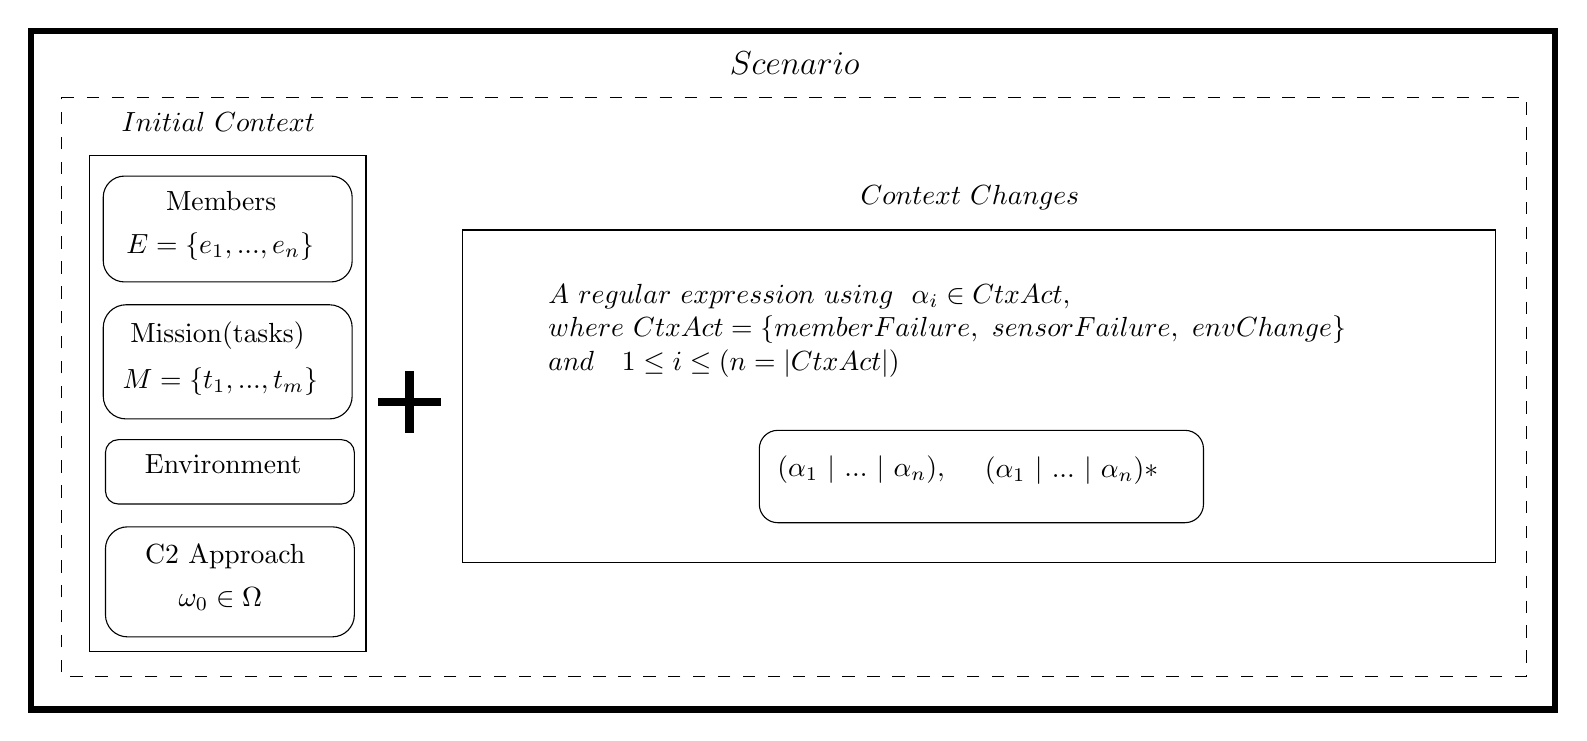
\begin{tikzpicture}[x=0.75pt,y=0.75pt,yscale=-1,xscale=1]
%uncomment if require: \path (0,349); %set diagram left start at 0, and has height of 349

%Rounded Rect [id:dp4190516071959901] 
\draw   (45.48,212.2) .. controls (45.48,208.78) and (48.25,206) .. (51.68,206) -- (159.2,206) .. controls (162.63,206) and (165.4,208.78) .. (165.4,212.2) -- (165.4,230.8) .. controls (165.4,234.22) and (162.63,237) .. (159.2,237) -- (51.68,237) .. controls (48.25,237) and (45.48,234.22) .. (45.48,230.8) -- cycle ;
%Rounded Rect [id:dp916271795400267] 
\draw   (44.41,152) .. controls (44.41,145.92) and (49.34,141) .. (55.41,141) -- (153.34,141) .. controls (159.41,141) and (164.34,145.92) .. (164.34,152) -- (164.34,185) .. controls (164.34,191.08) and (159.41,196) .. (153.34,196) -- (55.41,196) .. controls (49.34,196) and (44.41,191.08) .. (44.41,185) -- cycle ;
%Rounded Rect [id:dp6771464113681669] 
\draw   (44.41,89.2) .. controls (44.41,83.57) and (48.98,79) .. (54.61,79) -- (154.14,79) .. controls (159.77,79) and (164.34,83.57) .. (164.34,89.2) -- (164.34,119.8) .. controls (164.34,125.43) and (159.77,130) .. (154.14,130) -- (54.61,130) .. controls (48.98,130) and (44.41,125.43) .. (44.41,119.8) -- cycle ;
%Shape: Rectangle [id:dp977819802873701] 
\draw   (37.75,69) -- (171,69) -- (171,308) -- (37.75,308) -- cycle ;
%Rounded Rect [id:dp11904903891609209] 
\draw   (45.48,258.6) .. controls (45.48,252.75) and (50.22,248) .. (56.08,248) -- (154.8,248) .. controls (160.66,248) and (165.4,252.75) .. (165.4,258.6) -- (165.4,290.4) .. controls (165.4,296.25) and (160.66,301) .. (154.8,301) -- (56.08,301) .. controls (50.22,301) and (45.48,296.25) .. (45.48,290.4) -- cycle ;

%Shape: Rectangle [id:dp6932811140385843] 
\draw  [dash pattern={on 4.5pt off 4.5pt}] (24.5,41) -- (730,41) -- (730,320) -- (24.5,320) -- cycle ;
%Shape: Rectangle [id:dp3952140034216508] 
\draw  [line width=2.25]  (9.5,9) -- (744,9) -- (744,336) -- (9.5,336) -- cycle ;
%Shape: Rectangle [id:dp32385330595430617] 
\draw   (217.5,105) -- (715,105) -- (715,265) -- (217.5,265) -- cycle ;
%Rounded Rect [id:dp9646271465434701] 
\draw   (360.5,210.4) .. controls (360.5,205.48) and (364.48,201.5) .. (369.4,201.5) -- (565.6,201.5) .. controls (570.52,201.5) and (574.5,205.48) .. (574.5,210.4) -- (574.5,237.1) .. controls (574.5,242.02) and (570.52,246) .. (565.6,246) -- (369.4,246) .. controls (364.48,246) and (360.5,242.02) .. (360.5,237.1) -- cycle ;

\draw  [line width=3]  (177,188) -- (207,188)(192,173) -- (192,203) ;

% Text Node
\draw (345,18) node [anchor=north west][inner sep=0.75pt]  [font=\large]  {$Scenario$};
% Text Node
\draw (393,287) node [anchor=north west][inner sep=0.75pt]    {$\ \ $};
% Text Node
\draw (408,82) node [anchor=north west][inner sep=0.75pt]    {$Context\ Changes$};
% Text Node
\draw (52,47) node [anchor=north west][inner sep=0.75pt]    {$Initial\ Context$};
% Text Node
\draw (251,128) node [anchor=north west][inner sep=0.75pt]    {$ \begin{array}{l}
A\ regular\ expression\ using\ \ \alpha _{i} \in CtxAct,\ \\
where\ CtxAct=\{memberFailure,\ sensorFailure,\ envChange\} \ \\
and\ \ \ 1\leq i\leq ( n=|CtxAct|)
\end{array}$};
% Text Node
\draw (73.42,85) node [anchor=north west][inner sep=0.75pt]   [align=left] {Members};
% Text Node
\draw (56.17,148) node [anchor=north west][inner sep=0.75pt]   [align=left] {Mission(tasks)};
% Text Node
\draw (63.24,212) node [anchor=north west][inner sep=0.75pt]   [align=left] {Environment};
% Text Node
\draw (54.32,105) node [anchor=north west][inner sep=0.75pt]    {$E=\{e_{1} ,...,e_{n}\}$};
% Text Node
\draw (52.42,170) node [anchor=north west][inner sep=0.75pt]    {$M=\{t_{1} ,...,t_{m}\}$};
% Text Node
\draw (63.37,255) node [anchor=north west][inner sep=0.75pt]   [align=left] {C2 Approach};
% Text Node
\draw (79.49,276) node [anchor=north west][inner sep=0.75pt]    {$\omega _{0} \in \Omega $};
% Text Node
\draw (463.41,213) node [anchor=north west][inner sep=0.75pt]    {$\ ( \alpha _{1} \ |\ ...\ |\ \alpha _{n}) *$};
% Text Node
\draw (363.5,212.4) node [anchor=north west][inner sep=0.75pt]    {$\ ( \alpha _{1} \ |\ ...\ |\ \alpha _{n}) ,$};


\end{tikzpicture}}
    \caption{Scenario comprising the initial context variables and a sequence of events that characterizes a dynamic context}
    \label{fig:scenario}
\end{figure}

\X{As shown in Section~\ref{sec:example}, a dynamic context represents all the possibilities of changes: i) in the members, through unavailability of any nature; ii) in the mission, with changes in the tasks to be performed, or iii) in the environment, with disturbances in any element of the environment where the members act. However, for evaluating the system’s response to changes in the context, we selected a set of significant events that cause device damage or degradation of any nature, or any feature of status interest, depending on the specific type of system under concern. Table~\ref{table:context_changes} lists the actions related to a sample of context changes, combined with the initial context used by the simulation. These actions occur during the simulation to create a dynamic scenario, resembling realistic settings. Onboard sensors perceive environmental changes in all members and reduce their capability to be employed in a mission.}

%Table~\ref{table:context_changes} lists the possible actions combined with the initial context used by the simulation. These actions occur during the simulation to create a dynamic scenario, resembling realistic settings. Environmental changes are perceived by onboard sensors in all members and cause a reduction of their capability to be employed in a mission.


\begin{table}[ht]
	\small
	\fontsize{10}{10}\selectfont
	\centering
	\caption{Context changes handled by the simulator with related actions in the CS and their impact level in the system}
	\label{table:context_changes}

	\begin{tabular}{p{0.16\linewidth}p{0.18\linewidth}p{0.1\linewidth}p{0.43\linewidth}}
	\hline
		 \textbf{Change}
		& \textbf{Action}
		& \textbf{Impact}
		& \textbf{Description}  \\ [1ex]
	\hline	\\ [-1ex] 
	Environment & \textit{envChange} & low & Weather conditions (e.g., luminosity, cloudiness) impacting the sensor's quality; \\[1ex]
	& & & Hazard level requiring changes in the UAV's behavior \\[5ex]
	Self & \textit{sensorFailure} & medium & Sensor onboard damage caused by any internal issue (\color{blue}e.g.\color{black}, electronic circuit damaged) \\[1ex]
	& \textit{memberFailure} & high & UAV out of operation due to serious damage (e.g., no fuel or battery, or taken down) \\[6ex]
	
	%Mission & addTasks & 1 & tasks addition or removal in the mission \\[5ex]
	\hline
	\end{tabular}
\end{table} 



With military domain experts' collaboration, we classify these context change events according to their impact on the system. Such classification is based on consolidated doctrines of a situation analysis and planning in military operations with application in many different contexts~\citep{nato01, doctrine01, Fernandes2016, UAV_Aplication, CC03, UAV01}. It is used to create the sequences of events \color{black} in an increasing level of complexity\color{black}, requiring more resilience from the system. 

Table~\ref{tab:scenarios} shows the scenarios considered in the simulation. 
\color{black} The related event sequences were selected to have increasing level of complexity and commonality, based on the impact classification presented in Table~\ref{table:context_changes}, obtained from military domain experts. Accordingly, environment changes are more common to occur in the operation, followed by sensor issues and member failures because of enemy engagement or mechanical problems.
\color{black}

Besides the sequences of events presented, the initial contexts for all scenarios are formed by a team $E$ with 5 members, a mission $M$ with 30 tasks, and De-Conflicted as the initial C2 Approach $w_0$, i.e., a ring communication structure. During the simulation, these events occur in the sequence presented but at random times within the mission timeout.



\begin{table}[ht]
\centering
\fontsize{9}{9}
\selectfont
\caption{List of events (\textit{EC-envChange; SF-sensorFailure; MF-memberFailure}) that characterizes the context changes within the scenarios tested. The initial C2 Approach, the set of members $E$ and the mission $M$ remain unchanged.}
\label{tab:scenarios}
\begin{tabular}{|m{0.1\textwidth}|m{0.82\textwidth}|}
\hline
\rowcolor{lightgray}
 \textbf {Scenario} & \hfil  \textbf {Context Changes} \\
\hline  & \\[-1.5ex]
\hfil 1 & EC, EC, EC, EC, EC \\[1ex]
\hline  & \\[-1.5ex]
\hfil 2 & EC, EC, EC, EC, EC, EC, EC, EC, EC, EC, EC, EC, EC, EC, EC \\[1ex]
\hline & \\[-1.5ex]
\hfil 3 & 
EC, EC, EC, EC, EC, MF, EC, EC, EC, EC, EC, MF, EC, EC, EC, EC, EC, MF, EC, EC, EC, EC, EC  \\[1ex]
\hline & \\[-1.5ex]
\hfil 4 & EC, EC, EC, EC, EC, SF, EC, EC, EC, EC, EC, SF, EC, EC, EC, EC, EC, SF, EC, EC, EC, EC, EC  \\[1ex]
\hline & \\[-1.5ex]
 \hfil 5 & EC, EC, EC, SF, EC, EC, EC, MF, EC, EC, EC, SF, EC, EC, EC, MF, EC, EC, EC, SF, EC, EC, EC, MF  \\[1ex]
\hline & \\[-1.5ex]
 \hfil 6 & EC, SF, MF, EC, SF, EC, SF, EC, SF, MF, EC, SF, EC, SF, EC, SF \\[1ex]
\hline & \\[-1.5ex]
 \hfil 7 & MF, SF, EC, EC, EC, EC, EC, EC, EC, EC, EC, EC, MF, SF, EC, EC, EC, EC, EC, MF, SF, EC, EC, EC, MF, SF, EC \\[1ex]
 \hline & \\[-1.5ex]
 \hfil 8 & MF, SF, EC, MF, SF, EC, MF, SF, EC, MF, SF, EC \\[1.5ex]
 \hline & \\[-1.5ex] 
 \hfil 9 & SF, SF, SF, MF, SF, SF, SF, MF, SF, SF, SF, MF, SF, SF, SF \\[1ex]
 \hline & \\[-1.5ex] 
 \hfil 10 & SF, EC, MF, SF, EC, MF, SF, EC, MF, SF, EC, MF, EC, EC, EC, EC, EC, EC, EC, EC, EC, EC \\[1ex]
 \hline
\end{tabular}

\end{table}


The simulation operates a scenario with 5 possible types of tasks (0 to 4) and 5 types of sensors (A, B, C, D, and E). The tasks and onboard sensors are randomly chosen \color{black}before the round executes\color{black}. When the \color{black} task allocation \color{black}process starts, the algorithm applies a function that returns the quality $Q_{ij}$, obtained from a table, that correlates a sensor $i$ to the task $j$. When $Q_{ij}=0$ it means the sensor $i$ is not able to perform the task $j$.



%%%%%%%%%%%%%%%%%%%%%%%%%%%%%%%%%%
% SUBSECTION 
%%%%%%%%%%%%%%%%%%%%%%%%%%%%%%%%%%
\subsubsection{Experimental Design and Analysis Procedure}
\label{sssec:design}


Figure \ref{fig:exp_design} illustrates the factorial experimental design applied to assess the formulated hypotheses, where each action method is exercised with each scenario in a trial (cf. Section~\ref{sssec:scenarios}). Combinations of the factors are assessed with the metrics shown in Figure~\ref{fig:gqm}.


\begin{figure}[ht]
    \centering
    \scalebox{.6}{

\tikzset{every picture/.style={line width=0.75pt}} %set default line width to 0.75pt        

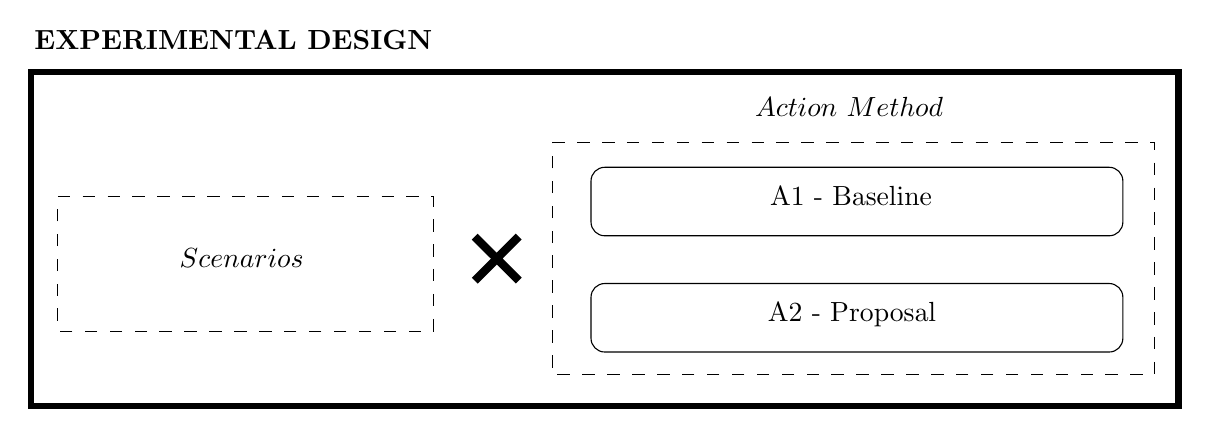
\begin{tikzpicture}[x=0.75pt,y=0.75pt,yscale=-1,xscale=1]
%uncomment if require: \path (0,201); %set diagram left start at 0, and has height of 201

%Rounded Rect [id:dp06575569211056953] 
\draw   (279.42,79.6) .. controls (279.42,75.95) and (282.37,73) .. (286.02,73) -- (529.06,73) .. controls (532.7,73) and (535.66,75.95) .. (535.66,79.6) -- (535.66,99.4) .. controls (535.66,103.05) and (532.7,106) .. (529.06,106) -- (286.02,106) .. controls (282.37,106) and (279.42,103.05) .. (279.42,99.4) -- cycle ;
%Shape: Rectangle [id:dp6932811140385843] 
\draw  [dash pattern={on 4.5pt off 4.5pt}] (22.5,87) -- (203.5,87) -- (203.5,152) -- (22.5,152) -- cycle ;
%Shape: Rectangle [id:dp9822494345299366] 
\draw  [dash pattern={on 4.5pt off 4.5pt}] (260.75,61) -- (551,61) -- (551,173) -- (260.75,173) -- cycle ;
%Shape: Rectangle [id:dp3952140034216508] 
\draw  [line width=2.25]  (9.5,27) -- (562.5,27) -- (562.5,188) -- (9.5,188) -- cycle ;
\draw  [line width=3]  (223.37,106.42) -- (244.63,127.58)(244.58,106.37) -- (223.42,127.63) ;
%Rounded Rect [id:dp9781270849297624] 
\draw   (279.42,135.6) .. controls (279.42,131.95) and (282.37,129) .. (286.02,129) -- (529.06,129) .. controls (532.7,129) and (535.66,131.95) .. (535.66,135.6) -- (535.66,155.4) .. controls (535.66,159.05) and (532.7,162) .. (529.06,162) -- (286.02,162) .. controls (282.37,162) and (279.42,159.05) .. (279.42,155.4) -- cycle ;

% Text Node
\draw (80,111) node [anchor=north west][inner sep=0.75pt]    {$Scenarios$};
% Text Node
\draw (357.17,38) node [anchor=north west][inner sep=0.75pt]    {$Action\ Method$};
% Text Node
\draw (10,6) node [anchor=north west][inner sep=0.75pt]   [align=left] {\textbf{EXPERIMENTAL DESIGN}};
% Text Node
\draw (364.41,81) node [anchor=north west][inner sep=0.75pt]   [align=left] {A1 - Baseline};
% Text Node
\draw (363.41,137) node [anchor=north west][inner sep=0.75pt]   [align=left] {A2 - Proposal};


\end{tikzpicture}}
    \caption{Factorial experimental design, where each action method is exercised with each scenario.}
    \label{fig:exp_design}
\end{figure}


The simulation uses a set of random variables to define some elements during execution, such as UAVs’ and tasks’ positions, and sensors that the context event will affect. \X{A simulator} engine generates these random numbers based on seeds created in runtime. For a consistent comparison between the action methods A1 and A2, a fixed set of seeds within the same trial were used in order to have the same value of such variables \X{during each} experimentation round.

To proceed with data analysis and sample size definition, a confidence level of 95\% in all statistical calculations was used. Such confidence level brings a significant population mean estimation and an acceptable sampling error. A \emph{p-value} of 0.05 was used to perform statistical hypothesis testing. The choice of these parameters is based on the standard cutoff used in \color{black}previous works; e.g.,~\citet{CochranW.G.1983} and~\citet{Bruce2014}. \color{black}


%%%%%%%%%%%%%%%%%%%%%%%%%%%%%%%%%%
% SUBSECTION 
%%%%%%%%%%%%%%%%%%%%%%%%%%%%%%%%%%
\subsubsection{Instrumentation}
\label{sssec:instrumentation}

Following related research on C2 simulation~\citep{FRANCE2014, Fernandes2016, Stanton2007, c2-02} and on the use of roles as components of agents' implementation~\citep{agent0010, agent1}, the simulations were performed using an agent-based framework, in this case Repast Simphony~\citep{North2013, SIMUL01, ClaesWohlinPerRuneson2012}. Figure~\ref{fig:repast01} shows an execution screen of the implementation \color{black} with the parameter fields \color{black} that can be changed to create different experimental setups \color{black} and the panel \color{black} with the agents' execution field.

The simulation implements the three roles modelled by the PGs shown in Figures \color{black} \ref{fig:ex_pg}, \ref{fig:ta_pg}, and \ref{fig:c2a_pg}  \color{black} to define UAV behavior with autonomy of reconfiguration, tasks allocation and execution, employed in a military recognition mission~\citep{UAV_Aplication}. Furthermore, perturbations and factors modifications were inserted in runtime to provide dynamism to the system and make it closer to a real scenario. A context change simulated by the system causes the quality reduction of a specific type of sensor, e.g., an environment change simulating a luminosity decreasing \color{black} reduces by $50\%$ \color{black} the quality of the sensor type 2 that represents a VGA camera. Sensor failure is modelled by setting its quality to zero. Furthermore, a member \color{black} can be lost with, consequently, \color{black} all its onboard sensors.

Inspired by the solution applied in~\citet{MAS07} and \citet{UAV01} to allocate tasks to a set of agents, a similar principle was used in this work based on swarm strategy. Depending on the C2 Approach \color{black}operating\color{black}, the members are notified about the allocation performed and unfinished tasks. This guarantees a better awareness level among entities and can improve the allocation result due to more context information shared by the members. Such allocation is feasible when a member has a configuration that activates a \color{black}task-compatible sensor\color{black}.

The C2 Approach \color{black}Maneuvering \color{black}follows the enumerated type described in Section~\ref{ssec:background_c2}. From the initial C2 Approach, which is De-Conflicted (cf. Section~\ref{sssec:scenarios}), the maneuver follows incrementally over this list and going back to Conflicted after Edge. The Conflicted is the final C2 Approach adopted by the system before discarding the unfeasible tasks. Such sequence is based on real scenarios of the military domain where a disconnected structure is adopted in extreme situations where there are no conditions to hold another communication and interaction strategy.


\begin{figure}[ht]
  \centering
  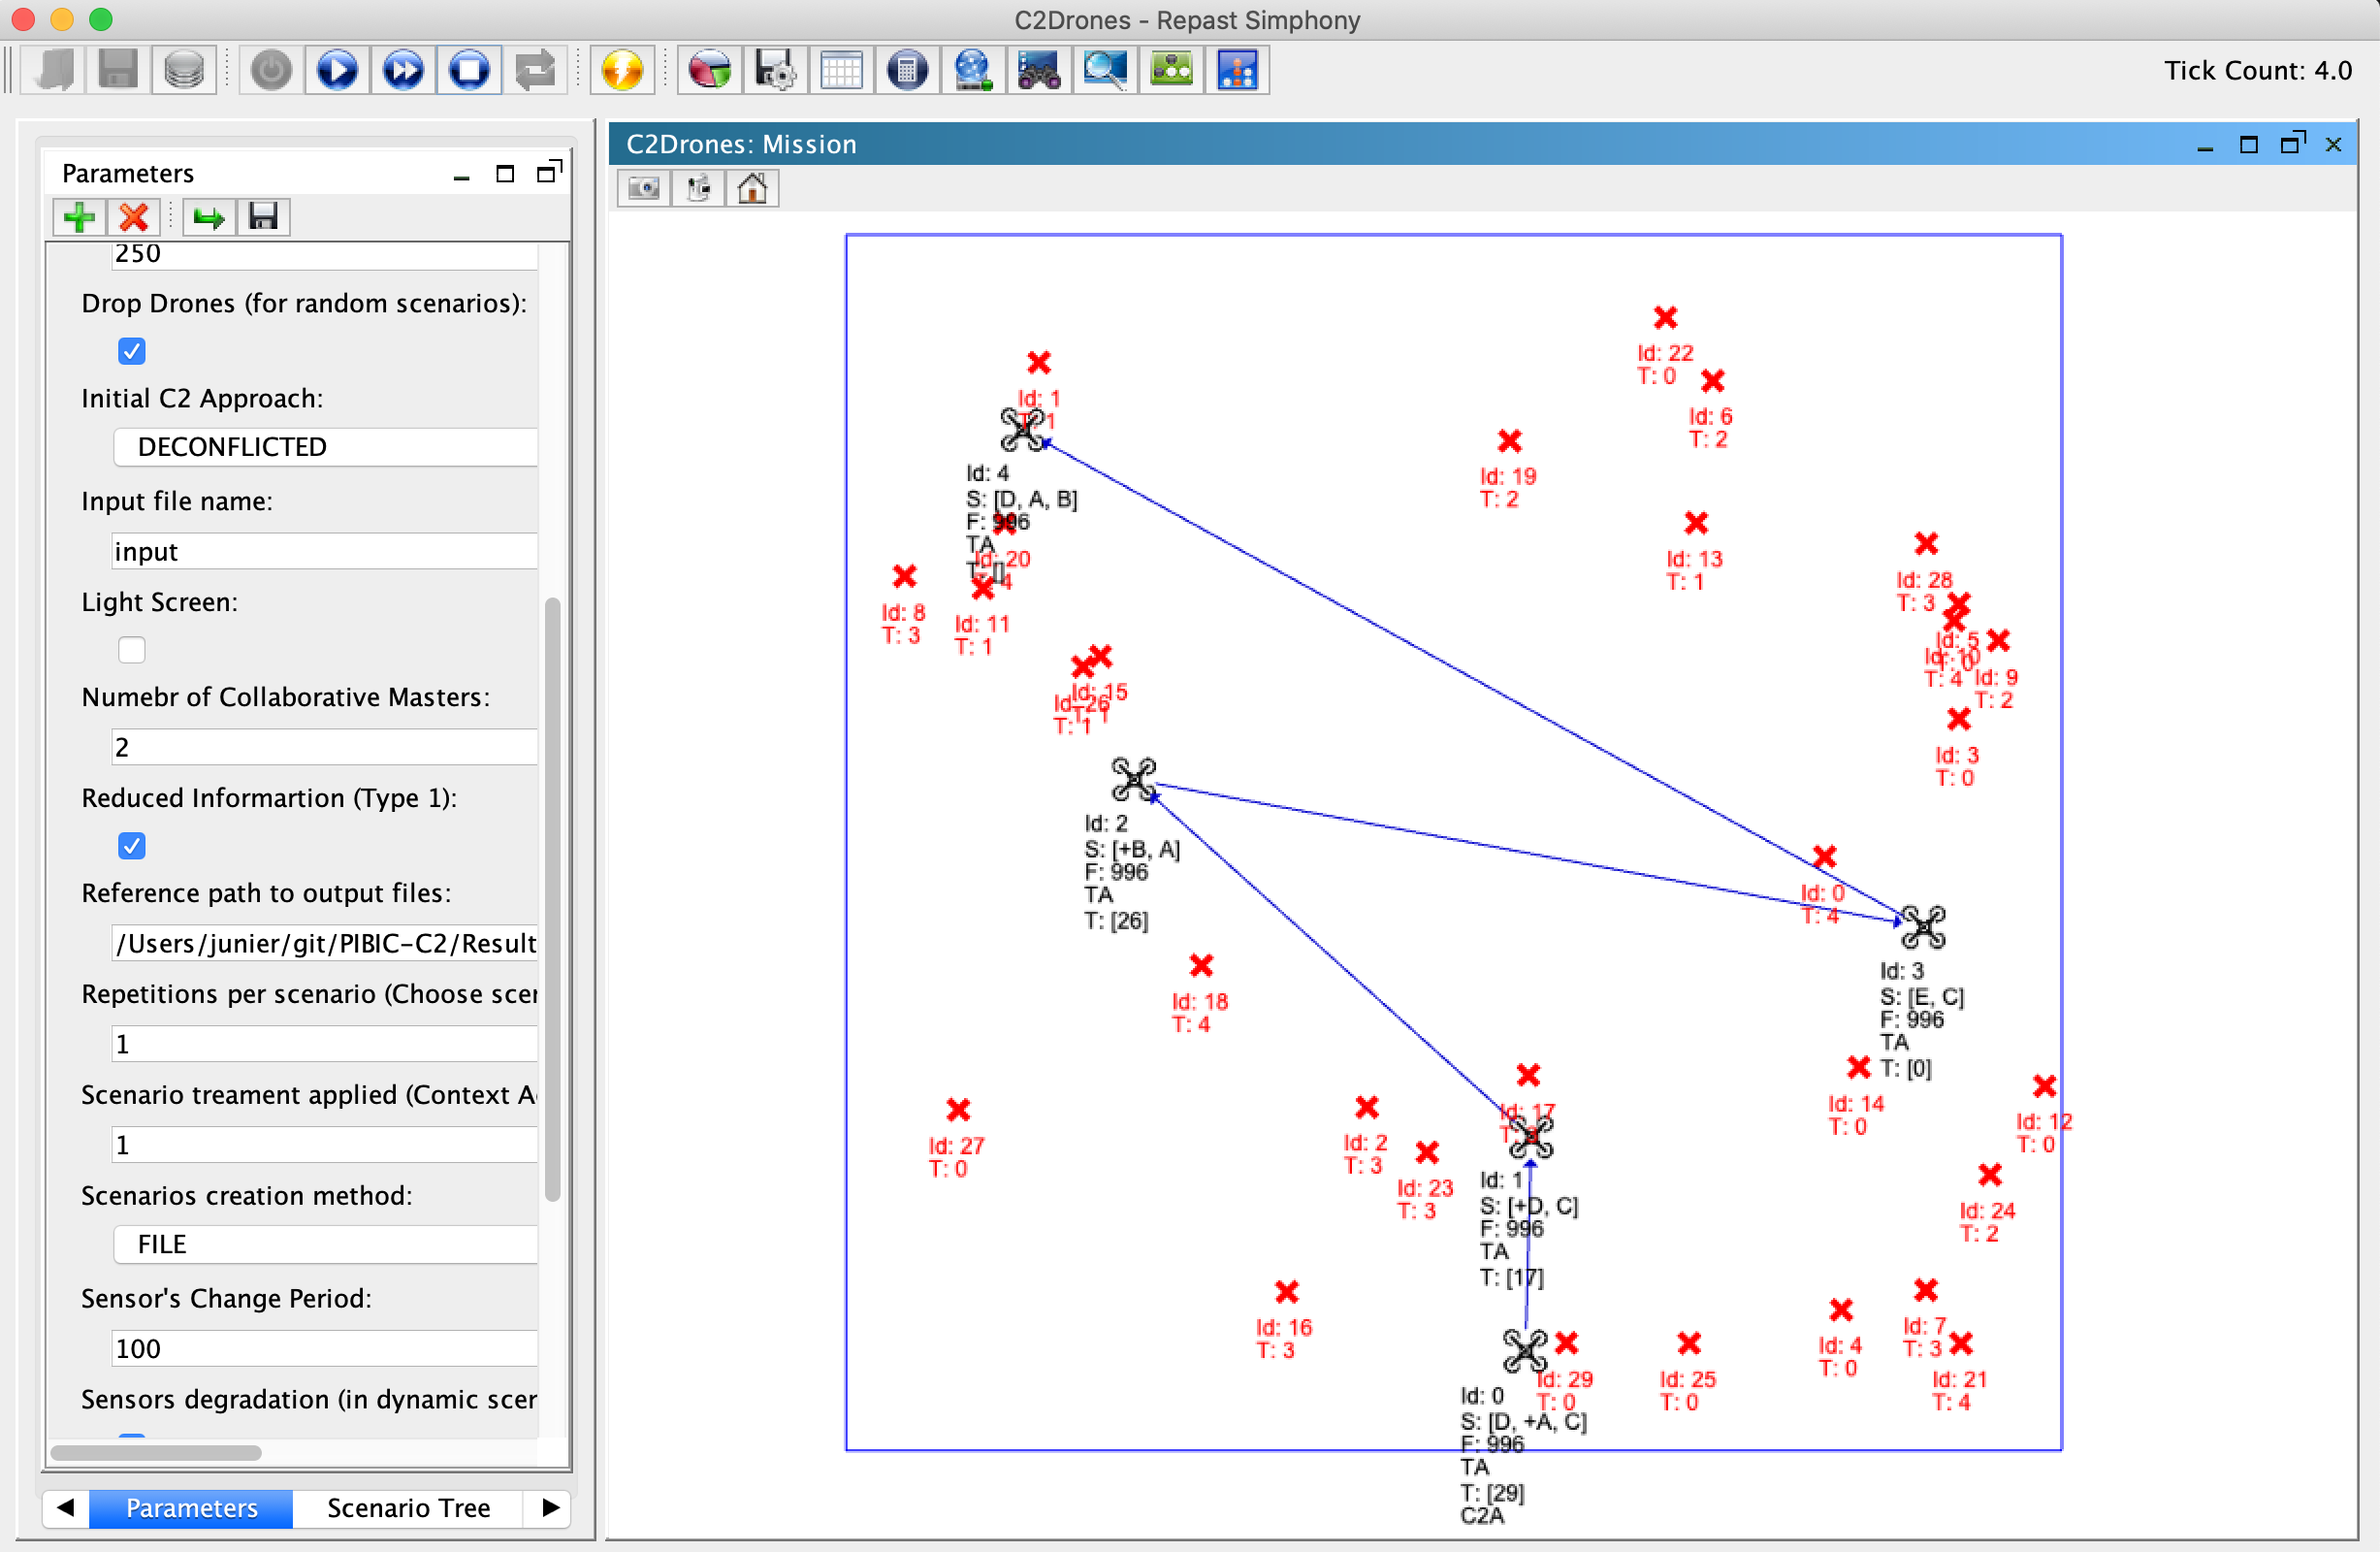
\includegraphics[width=0.7\linewidth]{img/repast01.png}
  \captionof{figure}{Simulator implementation  with Repast Simphony~\citep{SIMUL01}}
  \label{fig:repast01}
\end{figure}


The trials are performed feeding the simulator with the scenario data (cf. Section~\ref{sssec:scenarios}) combined with the two action methods shown in Figure~\ref{fig:exp_design}. Such scenarios are loaded through an input text file (CSV pattern). With all these data, the simulator runs each scenario with each action method, according to the experimental design (cf. Section~\ref{sssec:design}). The results are exported as text files and processed with \X{the R tool}~\citep{stat002,R_G} to calculate the mean and the standard deviation, draw graphs, and perform the statistical tests and validation.


%%%%%%%%%%%%%%%%%%%%%%%%%%%%%%%%%%
% SUBSECTION 
%%%%%%%%%%%%%%%%%%%%%%%%%%%%%%%%%%
\subsection{Executions}
\label{subsec:operations}

The experiment performs a significant set of executions in a batch way to reduce the effect of system startup on the standard deviation. An initial number of runs ($n_i=50$) was chosen to analyze the amount of dispersion in the results obtained by the experiments. Based on this, it was possible to observe the need to adjust the sample size to meet the acceptable confidence level (cf. Section~\ref{sssec:design}). According to \citet{CochranW.G.1983}, Equation~\ref{eq:stat} gives the sample size \emph{n} that satisfies a given confidence level, a population standard deviation $\sigma$, and the difference \emph{d} between the population mean ($\overline{X}$) and sample mean ($\mu$).

\begin{equation}
    \label{eq:stat}
    n=\left(\frac{Z_{\alpha/2} \cdot \sigma}{d}\right)^2
\end{equation}

According to the analysis procedure (cf. Section ~\ref{sssec:design}), the Equation~\ref{eq:stat} is applied with $95\%$ confidence, i.e., a $Z_{\alpha/2} = 1.96$, and $d = |\overline{X} - \mu| \leq 0.1\mu_i$, where $\mu_i$ is the mean obtained with the initial set of runs $n_i$. This value of $d$ is less than 10\% of the mean result obtained by the initial sample. With such parameters, an average sample size of 500 was obtained. Based on this, the factorial experiment with scenario and action method factors (see Figure~\ref{fig:exp_design}) was executed 500 times for all combinations of treatments. Table~\ref{table:results01} shows the results obtained for the metrics listed in GQM (Figure~\ref{fig:gqm}) for each scenario, which was performed 500 times. 

\begin{table}[ht]
	\small
	\fontsize{6.5}{6.5}\selectfont
	\centering
	\caption{Metrics results (Reconfigurations-M1, Maneuvering-M2, Engagement Time-M3, Effectiveness-M4, Resilience-M5 and Reward-M6)  after 500 executions of each scenario listed in Table~\ref{tab:scenarios} with the initial context of 5 members, 30 tasks, De-Conflicted as initial C2 Approach and a deadline of \color{black}1000 time ticks.\color{black}}
	\label{table:results01}
	
	\begin{tabular}{rrrrrrrr} \hline 
	    & \bf{M1}
		& \bf{M2}
        & \bf{M3}
        & \bf{M4}
		& \bf{M5}
		& \bf{M6} \\  \hline 
		
		& Mean(St.Dev.)  & Mean(St.Dev.) & Mean(St.Dev.)  & Mean(St.Dev.) & Mean(St.Dev.) & Mean(St.Dev.)  \\ [1ex]
		
		\multicolumn{7}{l}{\textbf{$\longrightarrow$ Scenario 1 }} \\
	% Scenario  1 
\bf{A1}  & 0.0 ($\pm$0.0)  & 0.0 ($\pm$0.0)  & 890.0 ($\pm$66.8)  & 82.0 ($\pm$5.9) & 97.5 ($\pm$1.0) & 20.7 ($\pm$1.7)  \\
\bf{A2}  & 17.5 ($\pm$1.7)  & 1.7 ($\pm$0.3)  & 945.5 ($\pm$33.1)  & 97.7 ($\pm$2.9)  & 99.9 ($\pm$0.1)  & 26.5 ($\pm$1.2)  \\ [1ex]
	
	\multicolumn{6}{l}{\textbf{$\longrightarrow$ Scenario 2 }} \\
% Scenario  2 
\bf{A1}  & 0.0 ($\pm$0.0)  & 0.0 ($\pm$0.0)  & 866.5 ($\pm$72.3)  & 77.5 ($\pm$6.3)  & 92.2 ($\pm$1.7)  & 20.0 ($\pm$1.7)  \\
\bf{A2}  & 18.1 ($\pm$2.1)  & 2.6 ($\pm$0.6)  & 934.0 ($\pm$33.0)  & 95.2 ($\pm$4.2)  & 97.3 ($\pm$1.3)  & 25.1 ($\pm$1.2)  \\ [1ex]
	
	\multicolumn{6}{l}{\textbf{$\longrightarrow$ Scenario 3 }} \\
% Scenario  3 
\bf{A1}  & 0.0 ($\pm$0.0)  & 0.0 ($\pm$0.0)  & 782.1 ($\pm$78.3)  & 63.7 ($\pm$5.5)  & 75.7 ($\pm$1.9)  & 16.1 ($\pm$1.3)  \\
\bf{A2}  & 15.4 ($\pm$1.7)  & 2.8 ($\pm$0.3)  & 883.0 ($\pm$49.2)  & 69.1 ($\pm$4.5)  & 70.7 ($\pm$2.3)  & 17.2 ($\pm$1.5)  \\ [1ex]
	
	\multicolumn{6}{l}{\textbf{$\longrightarrow$ Scenario 4 }} \\
% Scenario  4 
\bf{A1}  & 0.0 ($\pm$0.0)  & 0.0 ($\pm$0.0)  & 799.1 ($\pm$77.0)  & 63.6 ($\pm$5.3)  & 75.6 ($\pm$1.6)  & 16.4 ($\pm$1.3)  \\
\bf{A2}  & 18.2 ($\pm$2.3)  & 3.0 ($\pm$0.1)  & 913.4 ($\pm$35.9)  & 84.5 ($\pm$5.1)  & 86.4 ($\pm$2.4)  & 21.9 ($\pm$1.4)  \\ [1ex]
	
	\multicolumn{6}{l}{\textbf{$\longrightarrow$ Scenario 5 }} \\
% Scenario  5 
\bf{A1}  & 0.0 ($\pm$0.0)  & 0.0 ($\pm$0.0)  & 733.7 ($\pm$75.5)  & 54.6 ($\pm$4.6)  & 64.9 ($\pm$1.4)  & 13.9 ($\pm$1.2)  \\
\bf{A2}  & 16.1 ($\pm$2.0)  & 2.9 ($\pm$0.2)  & 887.7 ($\pm$48.4)  & 70.7 ($\pm$5.1)  & 72.3 ($\pm$2.9)  & 17.9 ($\pm$1.5)  \\ [1ex]
	
	\multicolumn{6}{l}{\textbf{$\longrightarrow$ Scenario 6 }} \\
% Scenario  6 
\bf{A1}  & 0.0 ($\pm$0.0)  & 0.0 ($\pm$0.0)  & 700.6 ($\pm$79.4)  & 42.0 ($\pm$4.5)  & 49.9 ($\pm$2.2)  & 10.7 ($\pm$1.1)  \\
\bf{A2}  & 15.0 ($\pm$2.0)  & 2.9 ($\pm$0.2)  & 910.5 ($\pm$59.3)  & 65.7 ($\pm$5.9)  & 67.2 ($\pm$3.9)  & 16.6 ($\pm$1.9)  \\ [1ex]
	
	\multicolumn{6}{l}{\textbf{$\longrightarrow$ Scenario 7 }} \\
% Scenario  7 
\bf{A1}  & 0.0 ($\pm$0.0)  & 0.0 ($\pm$0.0)  & 686.2 ($\pm$58.4)  & 41.1 ($\pm$3.5)  & 48.9 ($\pm$1.1)  & 10.9 ($\pm$1.0)  \\
\bf{A2}  & 15.0 ($\pm$2.0)  & 2.8 ($\pm$0.3)  & 820.5 ($\pm$61.4)  & 60.1 ($\pm$5.6)  & 61.5 ($\pm$3.7)  & 16.2 ($\pm$1.6)  \\ [1ex]
	
	\multicolumn{6}{l}{\textbf{$\longrightarrow$ Scenario 8 }} \\
% Scenario  8 
\bf{A1}  & 0.0 ($\pm$0.0)  & 0.0 ($\pm$0.0)  & 629.7 ($\pm$68.6)  & 36.3 ($\pm$3.8)  & 43.2 ($\pm$1.7)  & 9.1 ($\pm$0.9)  \\
\bf{A2}  & 13.0 ($\pm$1.5)  & 2.8 ($\pm$0.3)  & 785.1 ($\pm$58.3)  & 52.1 ($\pm$4.7)  & 53.3 ($\pm$3.1)  & 13.6 ($\pm$1.7)  \\ [1ex]
	
	\multicolumn{6}{l}{\textbf{$\longrightarrow$ Scenario 9 }} \\
% Scenario  9 
\bf{A1}  & 0.0 ($\pm$0.0)  & 0.0 ($\pm$0.0)  & 491.0 ($\pm$74.2)  & 26.4 ($\pm$3.7)  & 31.4 ($\pm$2.4)  & 7.0 ($\pm$1.0)  \\
\bf{A2}  & 15.5 ($\pm$1.6)  & 3.0 ($\pm$0.1)  & 743.2 ($\pm$66.1)  & 53.2 ($\pm$5.1)  & 54.4 ($\pm$3.4)  & 14.2 ($\pm$1.5)  \\ [1ex]
	
	\multicolumn{6}{l}{\textbf{$\longrightarrow$ Scenario 10 }} \\
		
% Scenario  10 
\bf{A1}  & 0.0 ($\pm$0.0)  & 0.0 ($\pm$0.0)  & 393.4 ($\pm$81.2)  & 24.3 ($\pm$2.6)  & 28.9 ($\pm$1.3)  & 6.2 ($\pm$0.9)  \\
\bf{A2}  & 11.4 ($\pm$1.4)  & 2.9 ($\pm$0.2)  & 650.7 ($\pm$114.8)  & 38.8 ($\pm$4.7)  & 39.7 ($\pm$3.4)  & 9.9 ($\pm$1.5)  \\ [1ex]
		\hline
	\end{tabular}
\end{table} 


%The simulation is not applying $addTask$ action due to the allocation task strategy adopted by the system, i.e., based on swarm algorithm, that puts the new task in the end of the available tasks list. Such position causes low impact in the system because the task will be allocated only if there is resources available after all previous allocation.


%%%%%%%%%%%%%%%%%%%%%%%%%%%%%%%%%%
% SUBSECTION 
%%%%%%%%%%%%%%%%%%%%%%%%%%%%%%%%%%
\subsection{Analysis and Discussion}
\label{subsec:analysis_discussion}


Table~\ref{table:results01} and Figures~\ref{fig:m1},~\ref{fig:m2},~\ref{fig:m3},~\ref{fig:m4},~\ref{fig:m5} and~\ref{fig:m6} show the results obtained by the simulation. Positive values for Reconfigurations (M1) (cf. Figure~\ref{fig:m1}) occur only in proposed method (A2) and indicates team's adaptation to deal with context changes in \color{black}all simulated scenarios\color{black}. By tracing into the source code of the simulation, we observed that such adaptations are followed by the tasks' reallocation activity in case the reconfiguration is not sufficient to make the member compatible with the task. A similar analysis can be applied to Maneuvering (M2) shown in Figure~\ref{fig:m2}. Positive values are obtained  only in the A2 method, which can perform a C2 Approach change to try a new awareness level. The values obtained show an upper bound due to the sequence of C2 Approach adopted starting from De-Conflicted up to Edge and finishing on the Conflicted one (cf. Section~\ref{ssec:background_c2}). 
%The values obtained show an upper bound due to the resource limitation to perform the mission, such as  members' fuel and time, which are spent during the C2 Approach change.

\begin{figure}
\centering
\begin{minipage}{.5\textwidth}
  \centering
  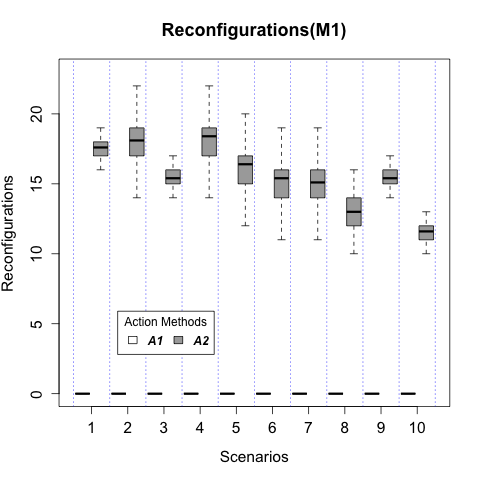
\includegraphics[width=0.95\linewidth]{img/graphs/Boxplot_M1.png}
  \captionof{figure}{Reconfigurations (M1)}
  \label{fig:m1}
\end{minipage}%
\begin{minipage}{.5\textwidth}
  \centering
  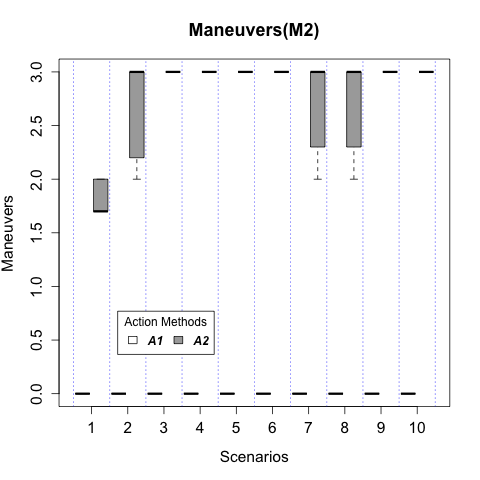
\includegraphics[width=0.95\linewidth]{img/graphs/Boxplot_M2.png}
  \captionof{figure}{Maneuvering (M2)}
  \label{fig:m2}
\end{minipage}
\end{figure}


Figure~\ref{fig:m3} shows results of Engagement Time (M3) for each scenario. In this case, the A2 method allows the system to keep running longer than A1, even in scenarios with more context changes. This suggests A2 provides more system availability due to its enhanced adaptation capability, as indicated by results for M1 and M2. 

 Regarding Effectiveness (M4), Figure~\ref{fig:m4} shows higher  capacity of the C2 system to solve tasks by the A2 method compared to A1, suggesting the higher availability obtained for M3 is well-employed in dealing with the mission in A2, increasing the system capacity to deal with context changes and to perform the tasks.


\begin{figure}
\centering
\begin{minipage}{.5\textwidth}
  \centering
  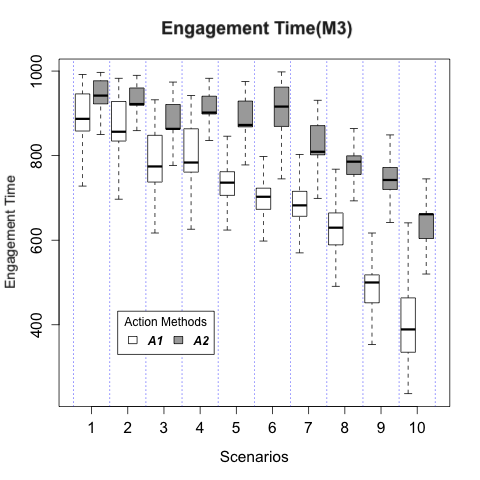
\includegraphics[width=0.95\linewidth]{img/graphs/Boxplot_M3.png}
  \captionof{figure}{Engagement time (M3)}
  \label{fig:m3}
\end{minipage}%
\begin{minipage}{.5\textwidth}
  \centering
  %  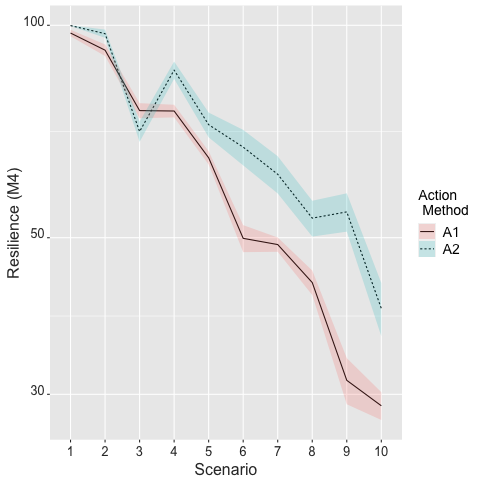
\includegraphics[width=0.95\linewidth]{img/graphs/Result_M4.png}
  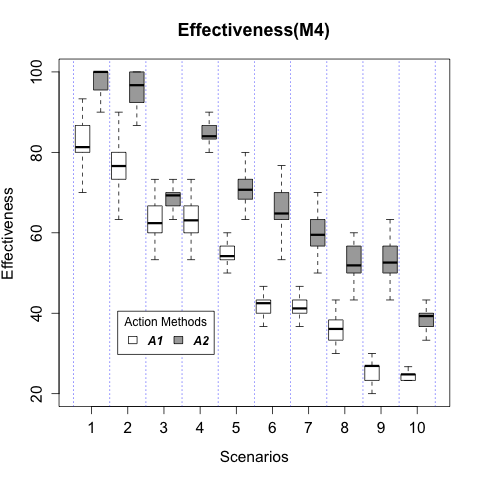
\includegraphics[width=0.95\linewidth]{img/graphs/Boxplot_M4.png}
  \captionof{figure}{Effectiveness (M4)}
  \label{fig:m4}
\end{minipage}
\end{figure}


Regarding the Resilience (M5) metric, Figure~\ref{fig:m5} shows that, in general, action method A2 is more capable of presenting a percentage of completed tasks closer to what would be obtained if the context remained unchanged. The only exception is for Scenario 3, since, upon exploration of simulation execution steps, the \emph{memberFailure} events in this scenario prompt task reallocation that cannot be better than the initial one made with the complete set of members. Besides, the time spent on members’ reconfiguration and tasks’ reallocation leads to a slightly lower result than that obtained by the A1 method, which only continues the execution.  

In terms of Reward (M6), Figure~\ref{fig:m6} shows better results for A2 indicating that the system adaptation provides more compatible configurations for performing tasks. Indeed, tracing into the simulation execution of method A2 reveals that all reconfiguration and C2 Approach change performed may lead to task reallocation. Such behavior always looks for the best member and sensor to perform the task to be allocated, reflecting the results presented in Figure~\ref{fig:m6}. In contrast, A1 performs only one allocation at mission startup. This way, when context change events occur, tasks are not \color{black}reallocated even when employed \color{black}sensors are damaged. Besides, if all 30 tasks in the mission are performed by the most compatible sensor for each one, i.e., with quality 1, we obtain the maximum result of 30 for reward (M6) metric. 
%Furthermore, as each sensor has a quality between 0 and 1 for each type of task, the maximum Reward metric (M6) that can be obtained is the sum of sensors' quality used, e.g., a total reward of 30 in a mission with 30 tasks using sensors with maximum quality level.



\begin{figure}
\centering
\begin{minipage}{.5\textwidth}
  \centering
  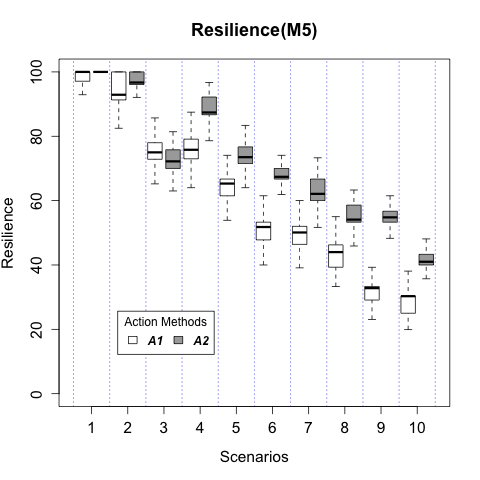
\includegraphics[width=0.95\linewidth]{img/graphs/Boxplot_M5.png}
  \captionof{figure}{Resilience (M5)}
  \label{fig:m5}
\end{minipage}%
\begin{minipage}{.5\textwidth}
  \centering
  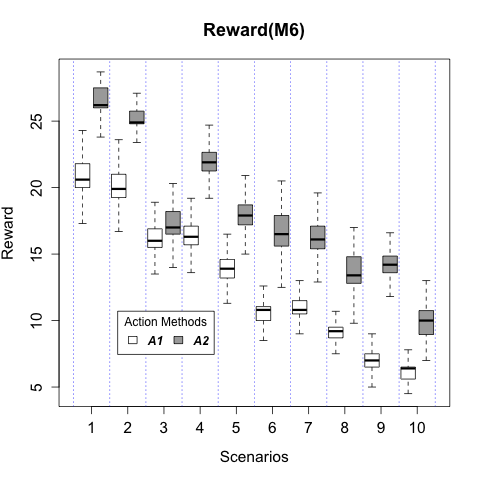
\includegraphics[width=0.95\linewidth]{img/graphs/Boxplot_M6.png}
  \captionof{figure}{Total reward (M6)}
  \label{fig:m6}
\end{minipage}
\end{figure}

Since removing members with the \emph{memberFailure} event does not allow members to reconfigure---prompting instead a task reallocation or even a C2 Approach change---it explains the decrease on M1, M4, M5, and M6 in Scenario 3 for method A2. \color{black}In contrast, \emph{sensorFailure} and \emph{envChange} enable member reconfiguration or change to the C2 Approach to search for an alternative allocation of pending tasks based on the algorithm used, i.e., swarm-gap based~\citep{MAS07, UAV01}, and the available context information. \color{black}It gives to A2 advantage in all other scenarios. Moreover, for methods A1 and A2, it is possible to observe a significant reduction in results for M3, M4, M5, and M6 due to the progressive loss of  system resources such as  members, sensors, and autonomy, as exercised by the scenarios. 

%Furthermore, the engagement time (M3) only suffered a significant decrease after a reduction in resources of more than 60\% identified from Scenario 6 onwards. 


%The \emph{null hypotheses $H_0$} in Table~\ref{table:hyp} can be refuted since the non-parametric statistical test demonstrated that the results of the metrics defined in GQM are different for the treatments applied to the action method. Even for Scenario 3, the \textit{p-value} for all metric were less than 0.05 and it indicates that the two samples compared, i.e., A1 and A2 results, are statistically different. Based on this, the alternative hypothesis is valid, confirming that the proposed method A2, able to perform internal reconfigurations and C2 Approach changes, presented a significant result in face of context changes simulated. We identify only Resilience (M5) metric in Scenario 3 with A1 results greater than A2 ones (cf. Figure~\ref{fig:m5}). These results evidence that the model proposed handles C2 Approach Agility (\emph{RQ1}) and C2 Maneuver Agility (\emph{RQ2}).

% Vander: after thinking about this the whole day, I fail to draw in my head any new info from comparing M3
% and M4. I suggest either simplifying a lot the following 3 paragraphs into a single one or
% removing the discussion. Operationally, I suggest: 1) consensus discussion; 2) Thiago writes the paragraph.
%
\color{black}
Nonetheless, even though both M3 and M4 decrease as scenarios become more complex, they do so at different rates.
Indeed, mean engagement time decreases less than 20\% before scenario 8, whereas mean effectiveness decreases about 46\% for the same scenarios (cf. Table~\ref{table:results01}).
This trend suggests that engagement time is not necessarily an indicator of effectiveness, strengthening the claim made by~\citet{Alberts2006} that ``the quality of C2 should not be deduced solely from mission outcomes''.
\color{black}


%The engagement time (M3) and the effectiveness (M4) metrics are complementary and highlights that the mission engaged does not show a direct ratio with its accomplishing. The main reason for this statement is the time spent by the entities to deal with context change, e.g., to find an appropriate allocation of remaining tasks. With the complexity of the events sequence that characterizes the context changes, it is possible to notice a significant reduction of M3, starting from scenario 7 as shown in Figure~\ref{fig:m3}, of about 40\% in the total time in ticks with our proposed model. Such decreasing is even bigger with no adaptation and coordination, i.e., with the action method A1. The context dynamism affects the M4 earlier, with a significant decreasing starting from scenario 3 (cf. Figure~\ref{fig:m4}) and getting up to 60\% of reduction in the percentage of completed tasks, in scenario 10.

%Even keeping long engagement in the mission, with negative impact only in complex scenarios with more change events, the overhead incurred by structure reorganization reduces the time for performing tasks. The number of C2 Approach changes (cf. Figure~\ref{fig:m2}), guided by the amount of context change events, causes reorganization of the members’ communication structure to continue executing the unfinished tasks and, because of this, causing a time-consuming. Based on this, comparing Figures~\ref{fig:m3} and~\ref{fig:m4}, we should have, conceptually, the engagement time in order to keep the effectiveness. However, we notice a time-consuming that reduces the number of complete tasks. In summary, the proposed modeling provided a higher percentage of mission completion (cf. Figure~\ref{fig:m4}), but there is a trade-off regarding the time taken to apply C2 agility.


%Even with a reduced decrease of less than 40\ when reaching the most complex scenario, i.e., the scenario 10, we faced a significant reduction of about 60\ in the effectiveness, i.e., the capacity of successfully executing tasks. In addition, comparing Figures~\ref{fig:m3} and~\ref{fig:m4}, we note a significant reduction of results in Scenarios 3 to 10 in the Engagement Time (M3) metric. These two scenarios present the maximum number of C2 Approach changes (cf. Figure~\ref{fig:m2}) because of the amount of context change events and the members’ need to reorganize the communication structure to continue executing the available tasks. Even keeping engaged in the mission, the overhead incurred by such reorganization reduces time for performing tasks. \color{black}

%Besides, as the members’ current task execution can be interrupted by a context change event, the effectiveness level (Figure~\ref{fig:m4}) drops faster than the engagement time (Figure~\ref{fig:m3}) since the total available execution time is limited by system’s resources and the mission execution deadline. Even with this decrease, it is possible to observe a considerable difference in these metrics’ values obtained with the system running the baseline action method A1 and the A2 proposed.
 


Although the difference between the results with action methods A1 and A2 for all scenarios and metrics is graphically observable, a statistical test was performed to confirm these differences. With a Shapiro-Wilk test~\citep{stat001}, a \textit{p-value} less than 0.05 was obtained, thus indicating a non-normal distribution. Accordingly, an Mann-Whitney U Test described in~\citet{stat002} was applied, i.e., Wilcoxon-test in R, to check differences among the samples of action methods A1 and A2 for all scenarios. According to the number and value of samples, the statistical analysis confirmed the difference between all results from A1 and A2 methods for all simulated scenarios. All  \emph{null hypotheses $H_0$} in Table~\ref{table:hyp} were then refuted in favor of the alternative hypotheses. A2 has statistically significant higher values for all metrics, except for Resilience (M5) in Scenario 3, in which case A1 has a 7\% higher value for the reasons discussed previously. Therefore, the simulation results provide evidence that the proposed model  provides C2 Approach Agility (\emph{RQ1}) and C2 Maneuver Agility (\emph{RQ2}).


\begin{center}
\fbox{\begin{minipage}{30em}
In summary, simulation results suggest that the proposed model exhibits C2 agility. Indeed, the system stays more time in action, completes more tasks and more compatible ones, resulting in higher resilience thereby better coping with context changes and perturbations in dynamic scenarios.

\end{minipage}}    
\end{center}



%%% REWRITING
%Despite the found evidence, this work presents some limitations that are related to the task allocation and the C2 Approach choice. The simulator performs a non-optimized task allocation and presents limited resilience in this process. Moreover, the selection of the C2 Approach occurs sequentially according to its communications structure. Such a choice does not take into account a previous analysis of the context. In this case, the several attempts of the C2 Approach have a cost in terms of operating time and onboard resources, impacting the obtained results.

%In addition, the C2 concepts are applied only in the computational environment, i.e., simulations. This application scenario may highlight restrictions to the extension of the proposed model to other domains and scenarios. Besides, the events that provide dynamism to the context considered in this work are suitable for UAV's operation scenarios. To extend the proposed model to other areas, making it more compatible with real scenarios, it is necessary to include new events that may impact the model's behavior and may require significant adjustments.





